\prefacesection{Assignment}


The initial steps of implementing a fuzzy logic system are as follows:
\begin{itemize}
	\item Crisp inputs are converted to set of fuzzy linguistic variable, linguistic terms and membership functions in what is known as fuzzification. 
	\item Based on a set of rules, an inference is made
	\item Lastly, defuzzification is implemented by using the membership functions to provide crisp results.
\end{itemize}
Linguistic variables are natural language values assigned to ranges of numeric inputs or outputs. These linguistic variables can have a set of real life terms to used to define a portion of the overall variable. For example, the linguistic variable \textbf{height} may have the terms {short, medium or tall etc.}. 

\section*{Linguistic Variables}
Based on the requirements of the system, linguistic variables need to be defined for the fuzzy logic system. We know that there are two input variables: "Level" and "Demand". Additionally, an output variable is specified to represent the command given to the pumping system, which will be defuzzified to a final crisp output. Each of these variables should be segmented into the appropriate terms. 
\subsection*{Level}
With this variable, five terms have been used to define the ranges of the level in the water. The terms are as follows: 
\textbf{Level(l) = {very\_low, low, average, high, very\_high}.}\\
The membership functions are based on the ranges specified in the assignment document. Level of the water in the tank can range from between 0 and 100. The type of membership functions used are trapezoidal and triangle. The trapezoidal function are used on the most extreme cases such as very\_low and very\_high and triangle are used on the low, average and high. See figure \ref{member1} for graphical representation.

\begin{figure}[ht]
	\begin{center}
		\advance\leftskip-3cm
		\advance\rightskip-3cm
		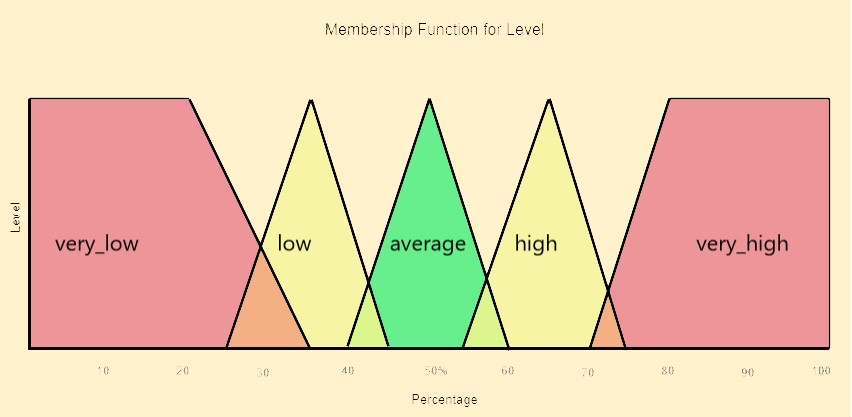
\includegraphics[keepaspectratio=true,scale=0.6]{__resources/level.jpg}
		\caption{Membership functions for Level}
		\label{member1}
	\end{center}
\end{figure}

\subsection*{Demand}
Like the level variable, five linguistic terms were made. The terms are as follows: \textbf{demand(d) = {very\_low, low, middle, high, very\_high}}. The demand variable has a range of -1 and 1.5. The same structure of two trapezoids and three triangle functions were used. 

\begin{figure}[ht]
	\begin{center}
		\advance\leftskip-3cm
		\advance\rightskip-3cm
		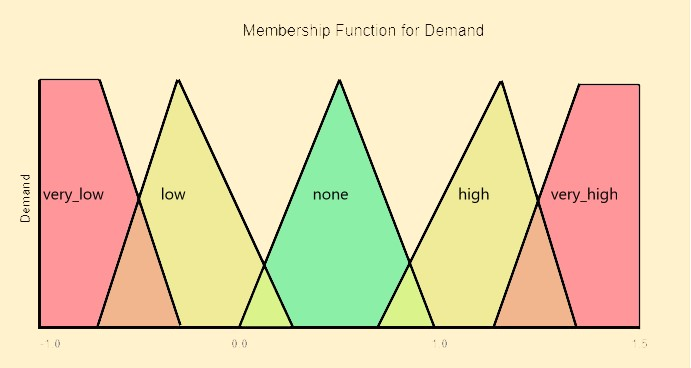
\includegraphics[keepaspectratio=true,scale=0.6]{__resources/demand.jpg}
		\caption{Membership functions for demand}
		\label{member2}
	\end{center}
\end{figure}


\newpage

\section*{Rule Terms}
in order to establish an output variable a set of rules must be defined control the value of the output variable. The three terms used for the output variable are as follows: \textbf{Command = {pump\_in, no\_pump, pump\_pump out}}. The following diagram shows the membership functions of the output variable command.
\begin{figure}[ht]
	\begin{center}
		\advance\leftskip-3cm
		\advance\rightskip-3cm
		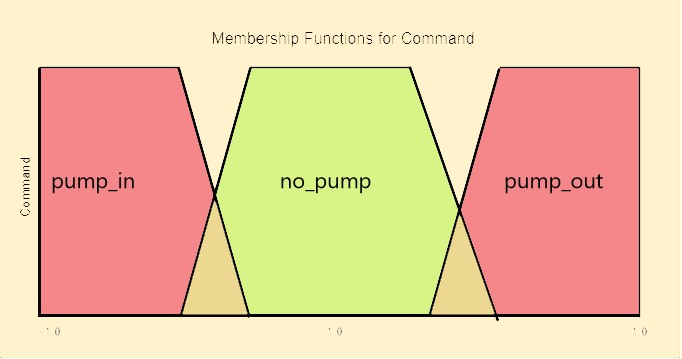
\includegraphics[keepaspectratio=true,scale=0.6]{__resources/command.jpg}
		\caption{Membership functions for command}
		\label{member2}
	\end{center}
\end{figure}
\newpage
A rule matrix will be utilized to illustrate the number of possible rules in the system. The top row signifies the demand variable with the terms it has been provided. Also, the first column displays the Level linguistic variable and it's terms. The intersection terms in the cells contain the command output variable that will be used to control the system.\\

\begin{tabular}{|c|c|c|c|c|c|}
	\hline 
	& \multicolumn{5}{c|}{\textbf{Demand}} \\ 
	\hline 
	\textbf{Level} & very\_low & low & middle & high & very\_high \\ 
	\hline 
	very\_low & pump\_in & pump\_in & pump\_in & pump\_in & no\_pump \\ 
	\hline 
	low & pump\_in & pump\_in & no\_pump & pump\_out & no\_pump \\ 
	\hline 
	average & no\_pump & no\_pump & no\_pump & pump\_out & pump\_out \\ 
	\hline 
	high & no\_pump & pump\_out & pump\_out & pump\_out & pump\_out \\ 
	\hline 
	very\_high & pump\_out & pump\_out & pump\_out & pump\_out & pump\_out \\ 
	\hline 
\end{tabular} \\\\
Following the implementation of the rule matrix, a set of rules need to be defined using an \textit{IF-THEN} format. 


 \begin{longtable}{|l|>{\raggedleft\arraybackslash}p{4cm}|l|l|l}
	\hline 
 	\multicolumn{4}{|l|}{IF (level is very\_low) and (demand is very\_low or low or middle or high) THEN command is pump\_in} \\ 
 	\hline 
 	\multicolumn{4}{|l|}{IF (level is very\_low) and (demand is very\_high) THEN command is no\_pump} \\ 
 	\hline 
 	\multicolumn{4}{|l|}{IF (level is low) and (demand is very\_low or low) THEN command is pump\_in} \\ 
 	\hline 
 	\multicolumn{4}{|l|}{IF (level is low) and (demand is high or very\_high) THEN command is pump\_out} \\ 
 	\hline 
 	\multicolumn{4}{|l|}{IF (level is average) and (demand is very\_low or low or middle) THEN command is no\_pump} \\ 
 	\hline 
 	\multicolumn{4}{|l|}{IF (level is average) and (demand is high or very\_high) THEN command is pump\_out} \\ 
 	\hline 
 	\multicolumn{4}{|l|}{IF (level is high) and (demand is very\_low) THEN command is no\_pump} \\ 
 	\hline 
 	\multicolumn{4}{|l|}{IF (level is high) and (demand is low or middle or high or very\_high) THEN command is pump\_out} \\ 
 	\hline 
 	\multicolumn{4}{|l|}{IF (level is very\_high) and (demand is very\_low or low or middle THEN command is pump\_out} \\ 
 	\hline
 	\multicolumn{4}{|l|}{IF (level is very\_high) and (demand is high or very\_high) THEN command is pump\_out} \\ 
 	\hline 
 \end{longtable}

After some experimentation with the rules, it appeared that the more rules that were applied, and the more complex the rules were, the worse the system performed. Therefore only four of the rules where kept in the final implementation. Using the check boxes, the controller maintains the level of water in the tank between the 40\% and 70\% requirement.
